\documentclass[12pt]{article}
\usepackage{amsmath}
\usepackage{amssymb}
\usepackage[letterpaper,top=0.85in,bottom=1in,left=0.75in,right=0.75in,centering]{geometry}
%\usepackage{fancyhdr}
\usepackage{enumerate}
%\usepackage{lastpage}
\usepackage{multicol}
\usepackage{graphicx}

\reversemarginpar

%\pagestyle{fancy}
%\cfoot{}
%\lhead{Math 1560}\chead{Test \# 1}\rhead{May 18th, 2017}
%\rfoot{Total: 10 points}
%\chead{{\bf Name:}}
\newcommand{\points}[1]{\marginpar{\hspace{24pt}[#1]}}
\newcommand{\skipline}{\vspace{12pt}}
%\renewcommand{\headrulewidth}{0in}
\headheight 30pt

\newcommand{\di}{\displaystyle}
\newcommand{\abs}[1]{\lvert #1\rvert}
\newcommand{\len}[1]{\lVert #1\rVert}
\renewcommand{\i}{\mathbf{i}}
\renewcommand{\j}{\mathbf{j}}
\renewcommand{\k}{\mathbf{k}}
\newcommand{\R}{\mathbb{R}}
\newcommand{\aaa}{\mathbf{a}}
\newcommand{\bbb}{\mathbf{b}}
\newcommand{\ccc}{\mathbf{c}}
\newcommand{\dotp}{\boldsymbol{\cdot}}
\newcommand{\bbm}{\begin{bmatrix}}
\newcommand{\ebm}{\end{bmatrix}}                   
                  
\begin{document}


\author{Instructor: Sean Fitzpatrick}
\thispagestyle{empty}
\vglue1cm
\begin{center}
\emph{University of Lethbridge}\\
Department of Mathematics and Computer Science\\
{\bf MATH 1410 - Tutorial \#1}\\
Wednesday, January 17
\end{center}
\skipline \skipline \skipline \noindent \skipline

\vspace*{\fill}



Some additional practice (copy these into your notes but \textbf{do not submit anything}):
\begin{enumerate}
\item Given $z=3-2i$ and $w=4+5i$, compute:
\begin{multicols}{5}
\begin{enumerate}
\item $z+w$
\item $3z-2\overline{w}$
\item $z^2$
\item $zw$
\item $\dfrac{\overline{z}}{w}$
\end{enumerate}
\end{multicols}

\item Compute the following powers of $i$:
\begin{multicols}{5}
\begin{enumerate}
\item $i^3$ \item $i^4$ \item $i^6$ \item $i^{-5}$ \item $i^{1410}$
\end{enumerate}
\end{multicols}
\item Convert from polar to rectangular form:
\begin{multicols}{4}
\begin{enumerate}
\item $z=3e^{i(\pi/6) } $ 
\item $z= 2e^{i(17\pi/4) }$ \item $z=5e^{i(-19\pi/6)}$ \item $z=1410e^{i(1410\pi) }$
\end{enumerate}
\end{multicols}
\end{enumerate}




\newpage
%\thispagestyle{empty}

  \begin{enumerate}
    \item Solve the following equations for $z$:
    \begin{multicols}{2}
    \begin{enumerate}
    \item $\dfrac{3z}{5-2z} = 1+3i$
    
    
    
    \item $3z+(2-4i)\overline{z} = 4+5i$

    
    

    \end{enumerate}
        \end{multicols}
        
        \vspace{2.5in}
        
  \end{enumerate}
  \begin{multicols}{2}

  \begin{enumerate}
    \addtocounter{enumi}{1}
      \item A complex number $z$ is plotted on the right. On the same set of coordinate axes, also plot:
      \begin{multicols}{2}
      \begin{enumerate}
      \item $2z$
      \item $\overline{z}$
      \item $z^2$
      \item $\dfrac{1}{z}$
      \end{enumerate}
      \end{multicols}
      Your plots do not have to be perfectly accurate and you do not have to explain your choices here, but you should be sure that you could explain them if asked to do so.
      \begin{center}
      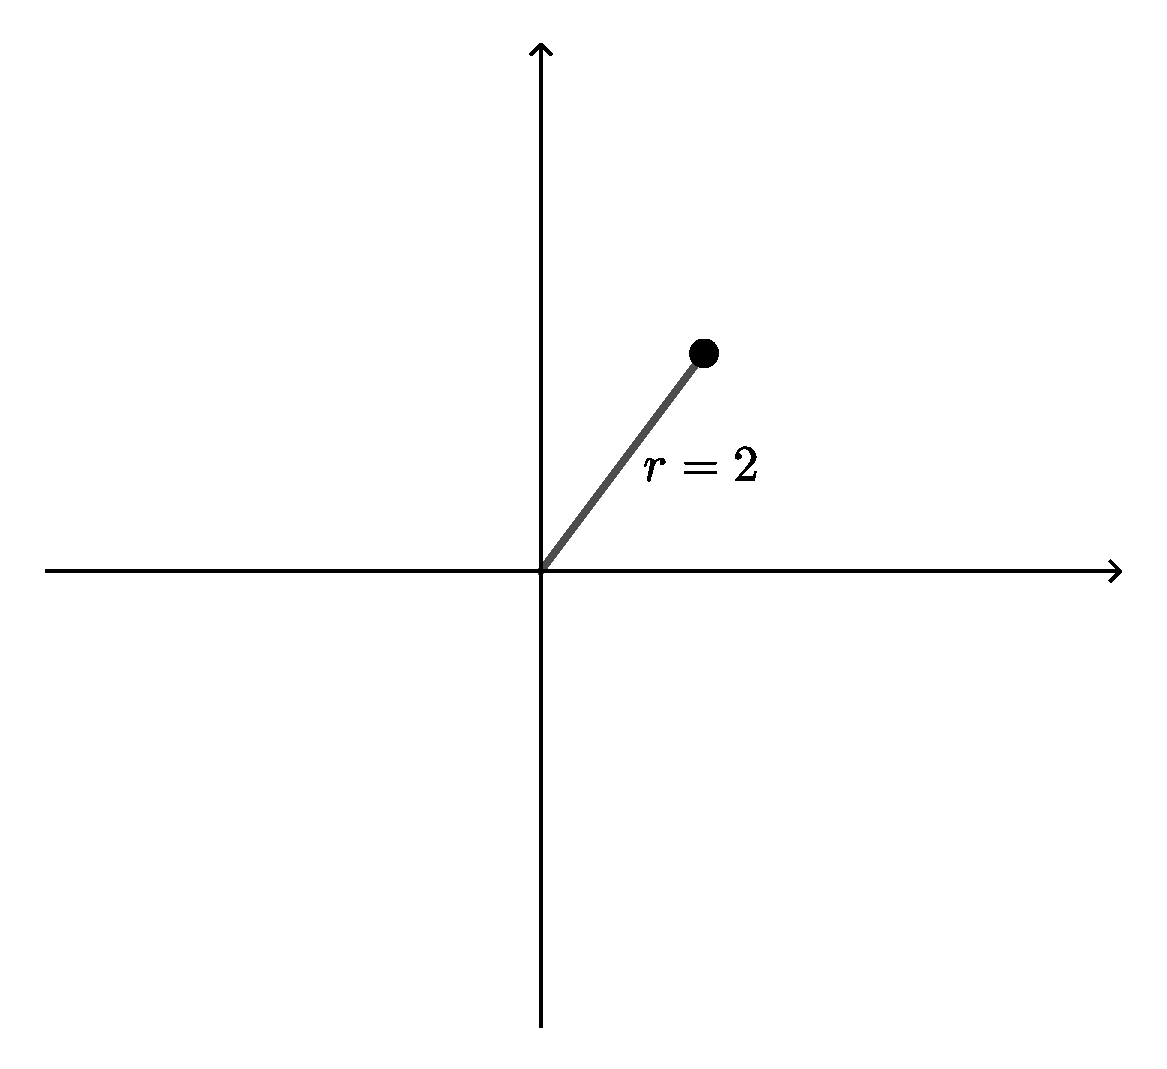
\includegraphics[width=0.8\columnwidth]{T1-2}
      \end{center}
  \end{enumerate}
\end{multicols}

\begin{enumerate}
\addtocounter{enumi}{2}
\item Convert $z=1-\sqrt{3}i$ to polar form, and compute the powers $z^7$ and $z^{-3}$.
\end{enumerate}
  
\end{document}